\chapter{Casos de Uso}
\section{Introduccion}
En base a lo que hemos revisado anteriormente nos damos cuenta que existen diferentes metodologías que nos permiten desarrollar software de calidad enfocadas a las necesidades que se tengan.
\\
\\
Dentro de un proyecto de software existen diferentes etapas, una de estas independientemente de la metodología que se esté utilizando es definir de manera concisa y general qué es lo que se quiere, ya que es fundamental para definir los requerimientos de software porque muchas veces lo que se plantea no es lo que realmente se ve en el proyecto terminado, es por esto que se definen formas de presentar una perspectiva primitiva de lo que será el software una vez finalizado.
\\
\\
Existen diferentes formas de representar la funcionalidad del software sin estar terminado,  una de estas es el Lenguaje Unificado de Modelado  “UML”, que  es el sistema de modelado de software más conocido y utilizado en la actualidad.



\newpage
Dentro de UML se pueden encontrar diversos diagramas que permiten representar las diferentes perspectivas de un sistema, ademas, apoyados en la herramienta Coloso se consiguio  el correcto modelado de dichos diagramas.
\\
\\
 Los Casos de Uso son diagramas que permiten representar que hará el sistema pero no como funciona, a continuación se analiza su implementación en nuestro proyecto de software.
\\
\\
\\
\\
\\
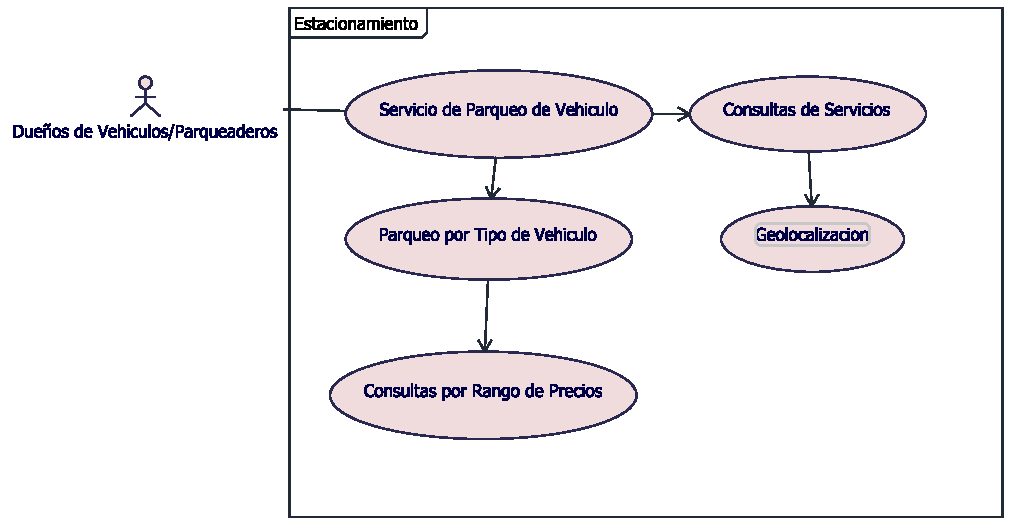
\includegraphics[width=1.25\linewidth]{imgs/Imagenes - casos de uso/Diagrama-General-Casos-de-Uso}
\\
\\
\\
\\
\\
\\
A continuacion, se realizaron una serie de tablas con descripciones de los casos de uso del diagrama anterior.
\newpage

\begin{longtable}{@{}|l|l|r@{}}
	\cmidrule(r){1-2}
	\multicolumn{2}{|c|}{Caso  uso: Servicio de Parqueo del Vehículo}&\\*
	\cmidrule(r){1-2}
	\endfirsthead
	\endhead
	\multicolumn{2}{|c|}{ 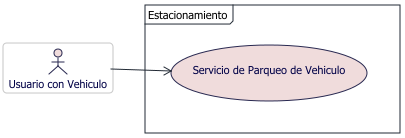
\includegraphics[width=0.5\linewidth]{imgs/Imagenes - casos de uso/Casoparqveh} }&
	\multicolumn{1}{l}{} \\* 
	\cmidrule(r){1-2}
	Descripcion  &Ubicar el vehículo en alguna plaza disponible.& \\* 
	\cmidrule(r){1-2}
	Actores &Usuario con vehículo, usuario con parqueadero.&\\* 
	\cmidrule(r){1-2}
	PreCondición &\begin{tabular}[c]{@{}l@{}}Ambos usuarios deben estar registrados, y el parqueadero debe\\ tener el estado disponible. \end{tabular} &\\* 
	\cmidrule(r){1-2}
	PosCondición &Se agrega el vehículo en el parqueadero y empieza a contabilizar el \\tiempo. &\\*
	\cmidrule(r){1-2}
	\multicolumn{2}{|c|}{Escenarios}& \\*
	\cmidrule(r){1-2}
	Primario& \begin{tabular}[c]{@{}l@{}}- Selecciono un parqueadero disponible en el área.\\- El dueño del parqueadero recibe una notificación de un nuevo \\vehículo.\\- Una vez llega el vehículo ambos usuarios confirman la llegada de\\ este.\\\end{tabular} &\\* 
	\cmidrule(r){1-2}
	Secundario   &\begin{tabular}[c]{@{}l@{}}- Selecciono un parqueadero no disponible.\\- Mostrará un aviso diciendo que este no se encuentra disponible\\\end{tabular}& \multicolumn{1}{l}{} \\* 
	\cmidrule(r){1-2}
	Excepcionales &\begin{tabular}[c]{@{}l@{}} -No hay parqueaderos disponibles.\\-  Le notificara que en esa área no es posible parquear su vehículo.\\\end{tabular} & 
	\multicolumn{1}{l}{} \\*
	\cmidrule(r){1-2}
\end{longtable}
\raggedleft
	Figura 0.0. Descripcion de caso de uso Servicio de \\Parqueo de 
	\centering Vehiculo"
	
\raggedleft
               
\newpage
\begin{longtable}{@{}|l|l|r@{}}
	\cmidrule(r){1-2}
	\multicolumn{2}{|c|}{Caso  uso: Parquear por tipo de vehículo}&\\*
	\cmidrule(r){1-2}
	\endfirsthead
	\endhead
	\multicolumn{2}{|c|}{ 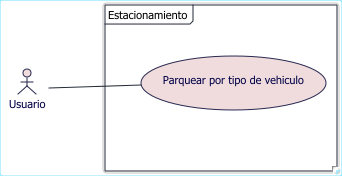
\includegraphics[width=0.5\linewidth]{imgs/Imagenes - casos de uso/Casoparqtipoveh} } &
	\multicolumn{1}{l}{} \\* 
	\cmidrule(r){1-2}
	Descripcion  & Clasificar los parqueaderos por tipo de vehículo soportado.& \\* 
	\cmidrule(r){1-2}
	Actores &Usuario con vehículo, usuario con parqueadero.&\\* 
	\cmidrule(r){1-2}
	PreCondición &\begin{tabular}[c]{@{}l@{}} Ambos usuarios deben estar registrados, el usuario con vehículo debe\\ tener el tipo de vehículo registrado  de igual manera el parqueadero \\el tipo de vehículo que pueden usarlo \end{tabular} &\\* 
	\cmidrule(r){1-2}
	PosCondición & Se mostrara si el parqueadero tiene plazas para el tipo de vehículo.&\\*
	\cmidrule(r){1-2}
	\multicolumn{2}{|c|}{Escenarios}& \\*
	\cmidrule(r){1-2}
	Primario& \begin{tabular}[c]{@{}l@{}}-Selecciono un parqueadero disponible en el área.\\ - Se mostrara si se puede usar este para su tipo de vehículo.\\\end{tabular} &\\* 
	\cmidrule(r){1-2}
	Secundario   &\begin{tabular}[c]{@{}l@{}}- Selecciono un parqueadero no compatible con el vehículo \\- No permitirá registrar el parqueo y volverá a la búsqueda. \\\end{tabular}& \multicolumn{1}{l}{} \\* 
	\cmidrule(r){1-2}
	Excepcionales &\begin{tabular}[c]{@{}l@{}} - No hay parqueaderos disponibles para su tipo de vehículo.\\- Le notificara que en esa área no es posible parquear su vehículo.\\\end{tabular} & 
	\multicolumn{1}{l}{} \\*
	\cmidrule(r){1-2}
\end{longtable}
\raggedleft
Figura 0.0. Descripcion de caso de uso " Parqueo por Tipo 
\centering de Vehiculo"

\raggedleft
\newpage
\begin{longtable}{@{}|l|l|r@{}}
	\cmidrule(r){1-2}
	\multicolumn{2}{|c|}{Caso  uso: Consulta por Rango de Precios}&\\*
	\cmidrule(r){1-2}
	\endfirsthead
	\endhead
	\multicolumn{2}{|c|}{ 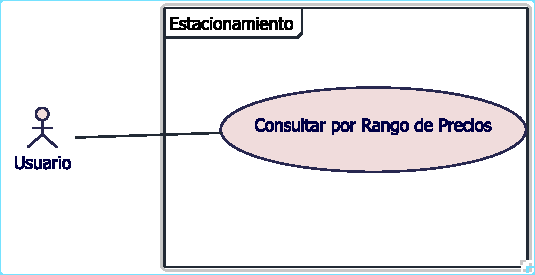
\includegraphics[width=0.5\linewidth]{imgs/Imagenes - casos de uso/Casofiltroprec} } &
	\multicolumn{1}{l}{} \\* 
	\cmidrule(r){1-2}
	Descripcion  &\begin{tabular}[c]{@{}l@{}}  Mostrar solo los parqueaderos que se encuentren en el rango \\de precios seleccionado por el usuario \end{tabular} & \\* 
	\cmidrule(r){1-2}
	Actores & Usuario con vehículo &\\* 
	\cmidrule(r){1-2}
	PreCondición & El usuario debe estar en el menú de búsqueda &\\* 
	\cmidrule(r){1-2}
	PosCondición & Solo se verán los parqueaderos filtrados por precio.&\\*
	\cmidrule(r){1-2}
	\multicolumn{2}{|c|}{Escenarios}& \\*
	\cmidrule(r){1-2}
	Primario& \begin{tabular}[c]{@{}l@{}}-Selecciono un rango de precios en el menú\\ - El mapa se actualizara mostrando solo los parqueaderos\\ que entran en ese rango \\\end{tabular} &\\* 
	\cmidrule(r){1-2}
	Secundario   &\begin{tabular}[c]{@{}l@{}}- Selecciono in rango de precios en el menú\\-No aparece ningún parqueadero en ese rango. \\- Se mostrara un mensaje diciendo que en esa área no hay \\parqueaderos dentro de ese rango de precios \end{tabular}& \multicolumn{1}{l}{} \\* 
	\cmidrule(r){1-2}
	Excepcionales &\begin{tabular}[c]{@{}l@{}} - -	El rango de precios seleccionado es de 0.\\- No se mostrara ningún parqueadero en el área. \\\end{tabular} & 
	\multicolumn{1}{l}{} \\*
	\cmidrule(r){1-2}
\end{longtable}
\raggedleft
Figura 0.0. Descripcion de caso de uso Consulta por rango de precios

\raggedleft

\newpage

\begin{table}[]
	\begin{tabular}{@{}|l|l|r@{}}
		\cmidrule(r){1-2}
		\multicolumn{2}{|c|}{Caso uso: Consultas de Servicios}                                                                                                             &                      \\ \cmidrule(r){1-2}
		\multicolumn{2}{|c|}{\begin{tabular}[c]{@{}c@{}}\\ 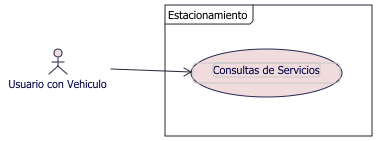
\includegraphics[width=0.6\linewidth]{imgs/Imagenes - casos de uso/Consultas} \\ \\ \end{tabular}}                                        & \multicolumn{1}{l}{} \\ \cmidrule(r){1-2}
		Descripcion  & \begin{tabular}[c]{@{}l@{}}Un sistema de consultas es aquel sistema digital que interactúa activamente \\con el usuario con dinámica conocida en relación con sus entradas y salidas\\ permitiendole hacer busquedas de todo tipo,\\ en funcion de su necesidad a partir de un servicio de parqueo adquirido.\end{tabular} &                      \\ \cmidrule(r){1-2}
		Actores       & Usuario con vehículo                                                                                                                              &                      \\ \cmidrule(r){1-2}
		PreCondición &       El Usuario debe haber adquirido un servicio de parqueo estar                                                                                                                        &                      \\ \cmidrule(r){1-2}
		PosCondición & \begin{tabular}[c]{@{}l@{}}                Se podra ver el resultado o la salida de la consulta hecha, relacionada \\  	  con el servicio     adquirido.                                                                                                           \end{tabular} &                     \\ \cmidrule(r){1-2}
		\multicolumn{2}{|c|}{Escenarios}                                                                                                            &                      \\ \cmidrule(r){1-2}
		Primario     & \begin{tabular}[c]{@{}l@{}}- Seleccion de un servicio adquirido \\- Recibo un tipo de consulta de un servicio adquirido\\ - Se recibe una consulta directa al usuario que presta el servicio\\\end{tabular}                                                                                &                      \\ \cmidrule(r){1-2}
		Secundario   &   \begin{tabular}[c]{@{}l@{}}- Se seleccionó una opcion no disponible   \\\end{tabular}                                                                                                                                & \multicolumn{1}{l}{} \\ \cmidrule(r){1-2}
		Excepcionales &   - Se selecciono una opcion sin haber solicitado previamente un servicio                                                                                                                           & \multicolumn{1}{l}{} \\ \cmidrule(r){1-2}
	\end{tabular}
\end{table}
\raggedleft
Figura 0.0. Descripcion de caso de uso Consulta de Servicios

\raggedleft

\newpage
\begin{table}[]
	\begin{tabular}{@{}|l|l|r@{}}
		\cmidrule(r){1-2}
			\multicolumn{2}{|c|}{Caso uso: Geolocalizacion real}                                                                                                             &                      \\ \cmidrule(r){1-2}
		\multicolumn{2}{|c|}{\begin{tabular}[c]{@{}c@{}}\\ 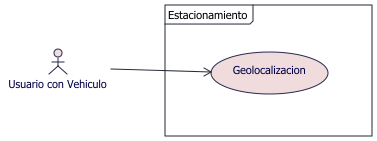
\includegraphics[width=0.6\linewidth]{imgs/Imagenes - casos de uso/Geolocalizacion} \\ \\ \end{tabular}}                                        & \multicolumn{1}{l}{} \\ \cmidrule(r){1-2}
		Descripcion  & \begin{tabular}[c]{@{}l@{}}La Geolocalización es un sistema que determina la ubicación de un objeto\\ en un entorno físico o virtual (Internet). A menudo, el objeto es una\\persona que quiere utilizar un servicio basado en la ubicación,\\ mientras mantiene su privacidad.\end{tabular} &                      \\ \cmidrule(r){1-2}
		Actores       & Usuario con vehículo                                                                                                                              &                      \\ \cmidrule(r){1-2}
		
		PreCondición &  \begin{tabular}[c]{@{}l@{}}    - El Usuario debe haber registrado su vehiculo \\- Haber seleccionado un servicio previamente \\- Haber dado los requeridos permisos de ubicacion                                                                                                                        \end{tabular}&                      \\ \cmidrule(r){1-2}
		
		PosCondición & \begin{tabular}[c]{@{}l@{}}               - Se podra seleccionar o visualizar directamente desde el mapa la \\ ubicacion deseada con las opciones previamente seleccionadas.                                                                                                           \end{tabular} &                     \\ \cmidrule(r){1-2}
		\multicolumn{2}{|c|}{Escenarios}                                                                                                            &                      \\ \cmidrule(r){1-2}
		
		Primario     & \begin{tabular}[c]{@{}l@{}}- Se genera un mapa de la zona con los requerimientos seleccionados \\- Se gestiona una solicitud de servicio\\\\\end{tabular}                                                                                &                      \\ \cmidrule(r){1-2}
		Secundario   &   \begin{tabular}[c]{@{}l@{}}- Se seleccionó una zona no disponible para visualizacion geo- espacial \\ - No hay disponibilidad para el servicio solicitado \\\end{tabular}                                                                                                                                & \multicolumn{1}{l}{} \\ \cmidrule(r){1-2}
		Excepcionales &\begin{tabular}[c]{@{}l@{}}   - Se selecciono la geolocalizacion sin haber solicitado previamente un \\servicio  \\- No fueron autorizados los permisos (ubicacion) requridos para el\\ funcionamiento de la herramienta    \end{tabular}                                                                                                                & \multicolumn{1}{l}{} \\ \cmidrule(r){1-2}
	\end{tabular}
\end{table}
\newpage